%REPORT TEMPLATE
%AUTHOR: RUI QU  
%EMAIL: RQU@KTH.SE 

%----------------------------------------------------------------------------------------
%	PACKAGES AND DOCUMENT CONFIGURATIONS
%----------------------------------------------------------------------------------------

\documentclass{article}

%---Basic---
\usepackage{natbib} % Required to change bibliography style to APA
\usepackage{amsmath} % Required for some math elements 
\setlength\parindent{0pt} % Removes all indentation from paragraphs
\usepackage{listings}%Insert code
\usepackage{times} % Uncomment to use the Times New Roman font

%---Table---
\usepackage{multirow}%Table
\usepackage{booktabs}%Table Triple-lines
\usepackage{siunitx} % Provides the \SI{}{} and \si{} command for typesetting SI units

%---Figure---
\usepackage{graphicx} % Required for the inclusion of images
\usepackage{subfigure} % Required for multiple images
\usepackage{float} 

%---Pseudo-code in LaTeX---
\usepackage{algorithm}
\usepackage{algpseudocode}
\usepackage{amsmath}
\renewcommand{\algorithmicrequire}{\textbf{Input:}}  % Use Input in the format of Algorithm
\renewcommand{\algorithmicensure}{\textbf{Output:}} % Use Output in the format of Algorithm

%---Appendix---
\usepackage{appendix}
\newcommand{\upcite}[1]{\textsuperscript{\textsuperscript{\cite{#1}}}} %Upcite

%----------------------------------------------------------------------------------------
%	DOCUMENT INFORMATION
%----------------------------------------------------------------------------------------

\begin{document}

\title{CS-E4950 Computer Vision\\Exercise Round 8}                  
\author{Rui Qu\\rui.qu@aalto.fi}
\maketitle

% If you wish to include an abstract, uncomment the lines below
% \begin{abstract}
% Abstract text
% \end{abstract}

%----------------------------------------------------------------------------------------
%	SECTION 1
%----------------------------------------------------------------------------------------

\section*{Exercise 1}



\textbf{c)} What could be the main reasons why most of the features are not tracked very long in case b) above?\\

Because the tracking algorithm will tracks liners and eliminate outliers from the last frame by using RANSCA. Key points will be missed when the image is rotated or the camera moves at a fast speed.\\

\textbf{d)} How could one try to avoid the problem of gradually losing the features? Suggest one or more improvements.\\

We try to avoid large movements over a short period of time so the system can learn new features and track them after a period of time.  Another try is to keep outliers rather than eliminating them for further tracking, but the problem is points always exist even if you move your face out of the camera. \\

\textbf{e)} 
\begin{figure}[H]
\centering  
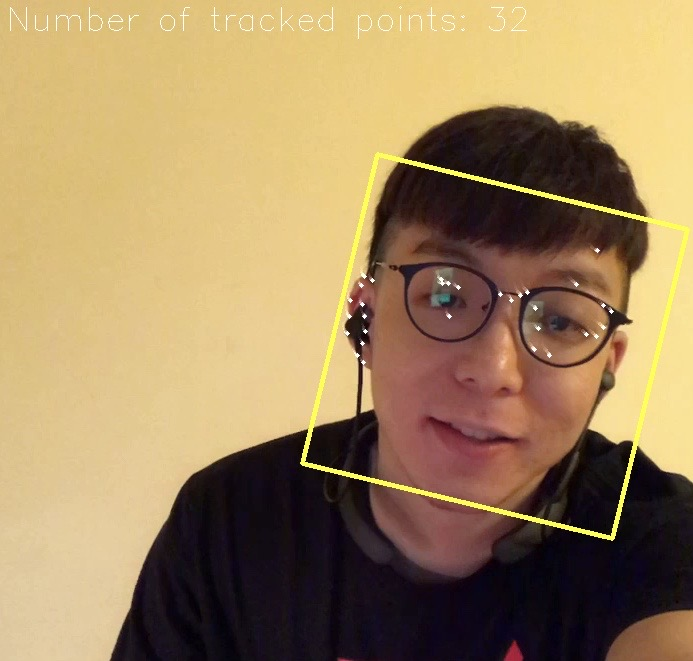
\includegraphics[scale=0.3]{1.png}
\caption{title}
\label{fig: label}
\end{figure}

\begin{figure}[H]
\centering  
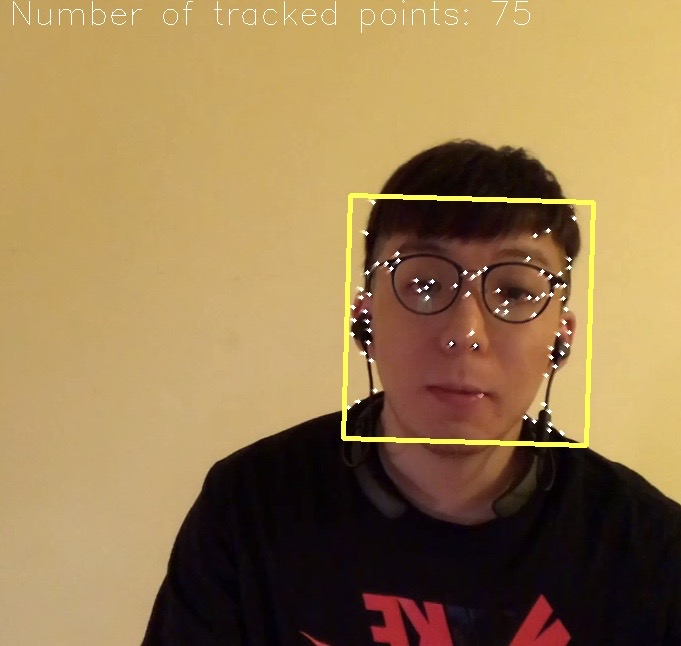
\includegraphics[scale=0.3]{2.png}
\caption{title}
\label{fig: label}
\end{figure}

\section*{Exercise 2}

%\nabla \top

Equation10 in the paper:
\begin{equation}
\Delta p= H^{-1}\sum_x \begin{bmatrix}\nabla I \frac{\delta W}{\delta p}\end{bmatrix}^{\mathsf{T}}\begin{bmatrix}T(x)-I(W(x;p))\end{bmatrix}
\end{equation}

where,
\begin{equation}
\begin{aligned}
&\frac{\delta W}{\delta p} = \begin{bmatrix}\frac{\delta W_x}{\delta u}&\frac{\delta W_x}{\delta v}\\ \frac{\delta W_y}{\delta u} & \frac{\delta W_y}{\delta v}  \end{bmatrix}=\begin{bmatrix}1&0\\0&1\end{bmatrix}\\
&\Delta P=\begin{bmatrix}u\\v \end{bmatrix}
\end{aligned}
\end{equation}

the Hessian matrix:

\begin{equation}
\begin{aligned}
H&=\sum_x \begin{bmatrix}\nabla I \frac{\delta W}{\delta p}\end{bmatrix}^{\mathsf{T}}\begin{bmatrix}\nabla I \frac{\delta W}{\delta p}\end{bmatrix}\\
&=\sum_x \begin{bmatrix}1&0\\0&1\end{bmatrix} \begin{bmatrix} \frac{\delta I}{\delta x}\\ \frac{\delta I}{\delta y} \end{bmatrix} \begin{bmatrix} \frac{\delta I}{\delta x}& \frac{\delta I}{\delta y} \end{bmatrix} \begin{bmatrix}1&0\\0&1\end{bmatrix}\\
&= \begin{bmatrix} \sum I_x I_x & \sum I_x I_y\\  \sum I_y I_x & \sum I_y I_y\end{bmatrix}
\end{aligned}
\end{equation}

Thus, Equation10 in the paper could be re-written:

\begin{equation}
\begin{aligned}
 \begin{bmatrix}u\\v \end{bmatrix}= \begin{bmatrix} \sum I_x I_x & \sum I_x I_y\\  \sum I_y I_x & \sum I_y I_y\end{bmatrix}^{-1}\sum_x \begin{bmatrix}I_x \\ I_y\end{bmatrix} \begin{bmatrix}T(x)-I(W(x;p))\end{bmatrix}
\end{aligned}
\end{equation}
which is the same as the equation in the slides:

\begin{equation}
\begin{aligned}
\begin{bmatrix} \sum I_x I_x & \sum I_x I_y\\  \sum I_y I_x & \sum I_y I_y\end{bmatrix} \begin{bmatrix}u\\v \end{bmatrix}= -\begin{bmatrix}\sum I_xI_y \\ \sum I_yI_t\end{bmatrix}
\end{aligned}
\end{equation}

  \begin{algorithm}[htb]
  \caption{ Framework of ensemble learning for our system.}
  \label{alg:Framwork}
  \begin{algorithmic}[1]
    \Require
      The set of positive samples for current batch, $P_n$;
      The set of unlabelled samples for current batch, $U_n$;
      Ensemble of classifiers on former batches, $E_{n-1}$;
    \Ensure
      Ensemble of classifiers on the current batch, $E_n$;
    \State Extracting the set of reliable negative and/or positive samples $T_n$ from $U_n$ with help of $P_n$;
    \label{code:fram:extract}
    \State Training ensemble of classifiers $E$ on $T_n \cup P_n$, with help of data in former batches;
    \label{code:fram:trainbase}
    \State $E_n=E_{n-1}cup E$;
    \label{code:fram:add}
    \State Classifying samples in $U_n-T_n$ by $E_n$;
    \label{code:fram:classify}
    \State Deleting some weak classifiers in $E_n$ so as to keep the capacity of $E_n$;
    \label{code:fram:select} \\
    \Return $E_n$;
  \end{algorithmic}
\end{algorithm}





\end{document}